\documentclass{beamer}
\usefonttheme[onlymath]{serif}

\usepackage[utf8]{inputenc}
\usepackage[T1]{fontenc}
\usepackage{lmodern}
\usepackage[francais]{babel}

% For table
\usepackage{booktabs} % To thicken table lines
\usepackage{multirow}
\usepackage{amsmath}

\graphicspath{{img/}}


\mode<presentation> {
	\usetheme{ulaval}
	\setbeamercovered{invisible}
}

\logo{
	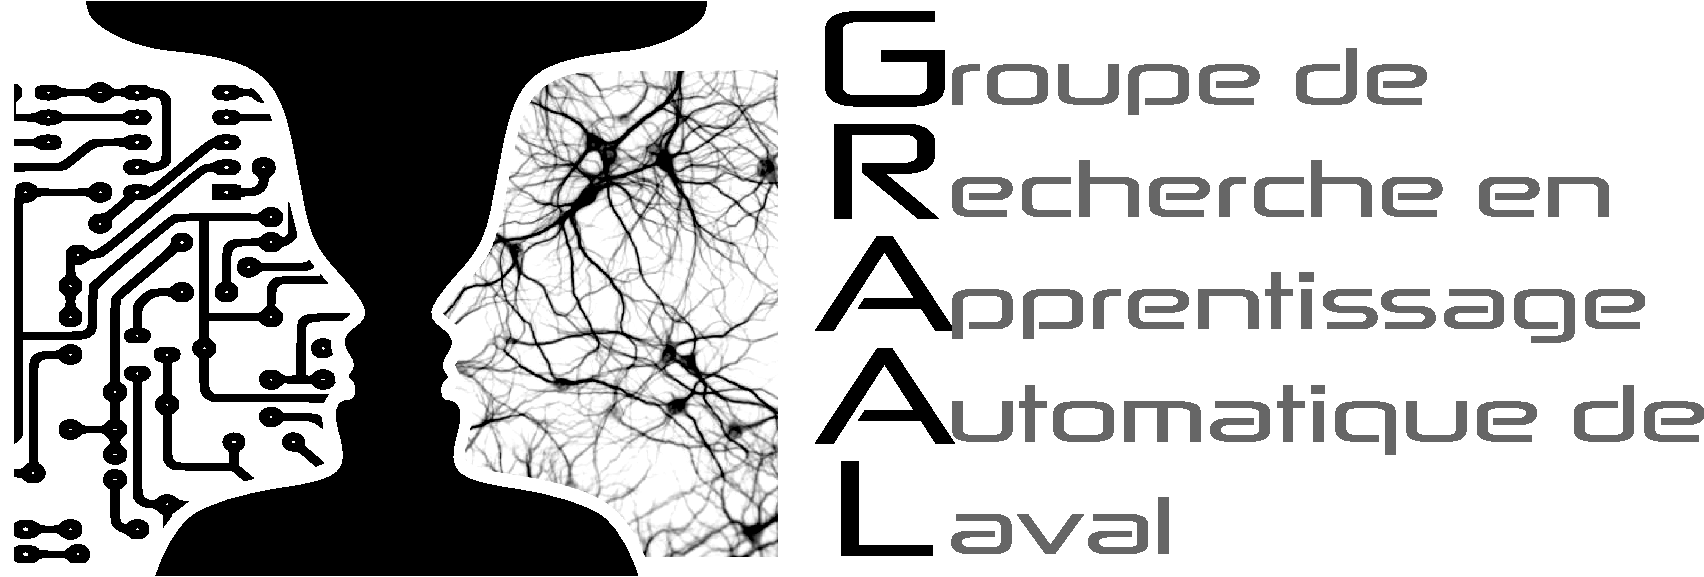
\includegraphics[height=0.65cm, keepaspectratio]{graal.pdf}\hspace{.2cm}\vspace{.85\paperheight}}


\title{Information gathering using external unstructured data sources}
%\subtitle[]{}

\author[D. Beauchemin]{David Beauchemin}
\institute[Université Laval]
{
	Département d'informatique et de génie logiciel, \\
	Université Laval\\
	\medskip
	{\emph{david.beauchemin.5@ulaval.ca}}
}
\date{\today}

\AtBeginSection[]
{
	\begin{frame}<beamer>
		\frametitle{Agenda}
		\tableofcontents[currentsection]
	\end{frame}
}

\begin{document}
	
	
	\begin{frame}[label=titre, plain]
		\titlepage
		\begin{center}
			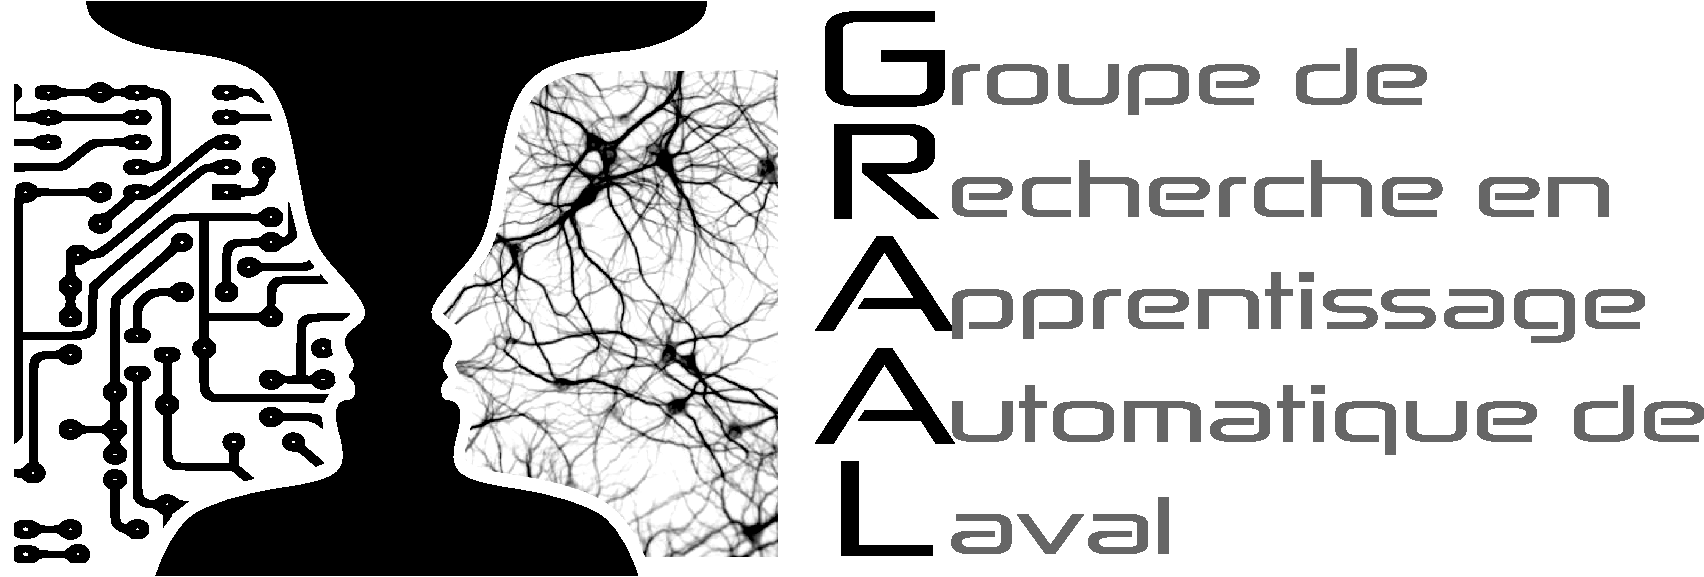
\includegraphics[height=1cm]{graal}
			
\includegraphics[height=1cm]{UL_P}
		\end{center}
	\end{frame}
	
	\section{Problématique de détection de doublons}
	
	\begin{frame}[label=intro]{Détection de doublons}
		\note{Explication rapide de la détection de doublons}
		\begin{center}
			\includegraphics[scale=1]{detection_doublons}
		\end{center}
	\end{frame}
	
	\section{Données}
	
	\subsection{Registre des entreprises du Québec (REQ)}
	
	\begin{frame}[label=REQ]\frametitle{Registre des entreprises du Québec (REQ)} 
		\begin{itemize}
			\item<1-> $\sim$3,5 millions d'entreprises
			\begin{itemize}
				\item Nom
				\item Adresse
				\item Activité économique
				\item Type d'enregistrement
			\end{itemize}
			\item<2-> $\sim$$36~\%$ des données sans adresse
			\item<3-> $\sim$$13~\%$ des données sans activité économique
			\item<4-> Possibilités que l'entité-vérité ne soit pas présente malgré l'annotation
		\end{itemize}
	\end{frame}
	
	\subsection{Yelp}
	
	\begin{frame}[label=Yelp]\frametitle{Yelp} 
		\begin{itemize}
			\item<1-> $\sim$193 000 entreprises en Amérique du Nord
			\begin{itemize}
				\item Nom
				\item Adresse
				\item Commentaires (\textit{classement})
			\end{itemize}
			\item<2-> $\sim$$27~\%$\note{50 644} des données au Canada
		\end{itemize}
	\end{frame}
	
	\subsection{Dun and Bradstreet}
	
	\begin{frame}[label=DunnBrad]\frametitle{Dun and Bradstreet} 
		\begin{itemize}
			\item<1-> 6 866 entreprises
			\begin{itemize}
				\item Nom
				\item Adresse
				\item Activité économique
			\end{itemize}
			\item<2-> $\sim$$14~\%$ (960) au Québec
			\item<3-> Jeux de données propriétaires
		\end{itemize}
	\end{frame}
	
	\subsection{Intact}
	
	\begin{frame}[label=intact]\frametitle{Intact} 
		\begin{itemize}
			\item<1-> 21 444 entreprises
			\begin{itemize}
				\item Nom
				\item Adresse
				\item Activité économique
			\end{itemize}
		\end{itemize}
	\end{frame}
	
	\begin{frame}[label=intact-REQ]\frametitle{Intact et REQ - Données utilisées} 
		\begin{itemize}
			\item<1-> 11 649 avec une adresse au Québec
			\begin{itemize}
				\item 580 annotés manuellement
				\begin{itemize}
					\item<2->  $19\%$ (108) sans adresse
					\item<2->  $17\%$ (100) négatifs
				\end{itemize}
				\item<3-> 50 données de validation pour l'approche par apprentissage automatique
				\begin{itemize}
					\item<4-> $18\%$ (9) sans adresse
					\item<4-> $14\%$ (7) négatifs
				\end{itemize}
			\end{itemize}
			\item<5-> $15\%$ des données du REQ ($\sim$300 000)
		\end{itemize}
	\end{frame}
	
	\begin{frame}[label=pretraitement-nom]\frametitle{Prétraitement des données utilisées} 
		Les méthodes de prétraitements sur le nom sont
		\begin{itemize}
			\item<1-> Normalisation via la mise en minuscule, le troncage des espaces en début et fin de nom et le retrait des accents.
			\begin{block}{Nom normalisé}
				\begin{center}
					L'Université Laval $\Rightarrow$ \textit{l'universite laval}
				\end{center}
			\end{block}
			\item<2-> À partir du nom normalisé on effectue le retrait des mots outils (i.e \textit{le}, \textit{la}, \textit{de})
			\begin{block}{Nom sans mot outil}
				\begin{center}
					l'universite laval $\Rightarrow$ \textit{'universite laval}
				\end{center}
			\end{block}
		\end{itemize}
	\end{frame}
	
	\begin{frame}[label=pretraitement-adresse]\frametitle{Prétraitement des données utilisées} 
		Les méthodes de prétraitements sur l'adresse sont
		\begin{itemize}
			\item<1-> Normalisation via la mise en minuscule, le troncage des espaces en début et fin de nom et le retrait des accents.
			\begin{block}{Adresse complète normalisée}
				\begin{center}
					2325 rue de l'Université, Québec, QC, G1V 0A6 \\ $\Downarrow$ \\ \textit{2325 rue de l'universite, quebec, qc, g1v 0a6}
				\end{center}
			\end{block}
			\item<2-> À partir de l'adresse normalisée on effectue regroupe les composantes de l'adresse par catégorie
			\begin{block}{Composantes de l'adresse}
				\begin{center}
					\scriptsize
					\begin{tabular}{cccc}
						\textbf{Numéro civique} & 2325                 & \textbf{Numéro d'unité} & $\emptyset$ \\
						\textbf{Nom de la rue}  & rue de l'universite, & \textbf{Code postal}    & g1v 0a6\\
						\textbf{Orientation}    & $\emptyset$                & &     \\
					\end{tabular}
				\end{center}
			\end{block}
		\end{itemize}
	\end{frame}
	
	\section{Déterminer la similarité entre deux entreprises}
	
	\subsection{Par mesure de similarité}
	
	\begin{frame}[label=sim]\frametitle{Par mesure de similarité}
		
		\note{Explication rapide de l'algorithme de couplage pas similarité}
		\begin{center}
			\includegraphics[scale=1]{sim_algo}
		\end{center}
		
	\end{frame}
	
	
	\subsubsection{Résultats du couplage du nom}
	
	\begin{frame}[label=distance-nom]\frametitle{Nom - Distance d'édition}
		\note{CCC très fort pour une approche naïve.
			Jaro et Jaro-Winkler mêmes résultats, hypothèse que début des phrases la similarité est pas si importante.
			Présence d'une sous séquence démontrer par PLSC.
			Nom sans mot outil vraiment meilleur.
		}
		\resizebox{\textwidth}{!}{%
			\begin{tabular}{ccccccc}
				\toprule
				\multicolumn{1}{l}{}                                                                                     & \multicolumn{1}{l}{} & CCC         & Levenhstein    & \multicolumn{1}{l}{Jaro} & \multicolumn{1}{l}{Jaro-Winkler} & \multicolumn{1}{l}{PLSC} \\ \midrule
				\multicolumn{1}{c}{\multirow{3}{*}{\begin{tabular}[c]{@{}c@{}}Nom normalisé\\ (\%)\end{tabular}}}      & Précision             & 99,56          & 74,94          & 90,86                     & 90,93                             & 85,40                    \\
				\multicolumn{1}{c}{}                                                                                   & Exactitude              & 56,38          & 51,55          & 68,10                     & 68,62                            & 67,41                     \\
				\multicolumn{1}{c}{}                                                                                   & Rappel                & 47,50          & 62,29          & 68,33                    & 68,96                             & 73,12                     \\ 
				\midrule
				\multicolumn{1}{c}{\multirow{3}{*}{\begin{tabular}[c]{@{}c@{}}Nom sans mot outil \\ (\%)\end{tabular}}} & Précision             & \textbf{99,58} & 75,19 & \textbf{90,33}                    & \textbf{90,49}                             & 85,37                    \\
				\multicolumn{1}{c}{}                                                                                   & Exactitude              & \textbf{57,76}          & 52,24 & \textbf{67,59}                     & \textbf{68,62}                             & 68,10           \\
				\multicolumn{1}{c}{}                                                                                   & Rappel                & \textbf{49,17} & 63,12 & \textbf{68,13}                     & \textbf{69,37}                    & 74,17           \\ \bottomrule
			\end{tabular}
		} % end of scope of "\resizebox"  directive
		\bigskip
		\begin{itemize}
			\item<2-> Résultats très bons malgré que l'on utilise des approches très simples.
			\item<3-> Le nom sans mot outil permet d'améliorer le couplage par le nom.
		\end{itemize}
		.
	\end{frame}
	
	\begin{frame}[label=jeton-nom]\frametitle{Nom normalisé - Jeton}
		\note{Sac de caractères n’apporte quasiment rien.
			Tous meilleurs que l'Approche naïve de CCC.
			Cosinus meilleure approche so far.
			Mais dans l'ensemble toutes les approches fonctionnent bien.
		}
		\begin{center}
			\begin{tabular}{cccccc}
				\toprule
				\multicolumn{1}{l}{}                                                                                     & \multicolumn{1}{l}{} & Jaccard & Cosinus        & \multicolumn{1}{l}{CSS} & \multicolumn{1}{l}{MASI} \\
				\midrule
				\multicolumn{1}{c}{\multirow{3}{*}{\begin{tabular}[c]{@{}c@{}}Sac de mots \\ (\%) \end{tabular}}}      & Précision             & \textbf{98,54}   & \textbf{92,46}          & 83,39                   & 98,73                    \\
				\multicolumn{1}{c}{}                                                                                   & Exactitude              & \textbf{63,10}   & \textbf{69,66}          & 49,83                   & 57,07                    \\
				\multicolumn{1}{c}{}                                                                                   & Rappel                & \textbf{56,25}   & \textbf{68,96}          & 49,17                    & 48,75                    \\ \midrule
				\multicolumn{1}{c}{\multirow{3}{*}{\begin{tabular}[c]{@{}c@{}}sac de caractères  \\ (\%) \end{tabular}}}      & Précision             & 74,49          & 76,80          & 0,00                     & 61,09                     \\
				\multicolumn{1}{c}{}                                                                                   & Exactitude              & 50,34          & 57,07          & 0,00                     & 27,07                     \\
				\multicolumn{1}{c}{}                                                                                   & Rappel                & 60,83          & 68,96         & 0,00                     & 32,71                     \\ \bottomrule
			\end{tabular}
		\end{center}
		\bigskip
		\begin{itemize}
			\item<2-> Cosinus et Jaccard sont très performant malgré leur simplicité.
			\item<3-> Le sac de caractères diminue grandement le couplage par le nom.
		\end{itemize}
	\end{frame}
	
	\begin{frame}[label=jeton-nom-outil]\frametitle{Nom sans mot outil - Jeton}
		\note{Sac de caractères apporte quasiment rien (encore).
			Tous meilleurs que l'Approche naïve de CCC.
			Cosinus meilleure approche so far.
			Jaccard et cosinus presque exactement les mêmes résultats qu'avec nom normalisé.
			Donc, dans l'ensemble le nom sans mot outil n'apporte pas vraiment une amélioration. Même que pour CSS diminue bcq les performances.
		}
		\begin{center}
			\begin{tabular}{cccccc}
				\toprule
				\multicolumn{1}{l}{}                                                                                     & \multicolumn{1}{l}{} & Jaccard & Cosinus        & \multicolumn{1}{l}{CSS} & \multicolumn{1}{l}{MASI} \\
				\midrule
				\multicolumn{1}{c}{\multirow{3}{*}{\begin{tabular}[c]{@{}c@{}}Sac de mots \\ (\%) \end{tabular}}}      & Précision             & \textbf{98,54}   & \textbf{92,22}          & 64,71                   & 98,78          \\
				\multicolumn{1}{c}{}                                                                                   & Exactitude              & \textbf{63,10}   & \textbf{69,66}          & 25,00                   & 58,62           \\ 
				\multicolumn{1}{c}{}                                                                                   & Rappel                & 56,25   & 69,17 & 20,62                    & 50,62           \\
				\midrule
				\multicolumn{1}{c}{\multirow{3}{*}{\begin{tabular}[c]{@{}c@{}}Sac de caractères  \\ (\%) \end{tabular}}} & Précision             & 75,06 & 77,01 & 0,99            & 61,39            \\ 
				\multicolumn{1}{c}{}                                                                                   & Exactitude              & 51,90 & 57,76 & 0,17            & 27,41            \\
				\multicolumn{1}{c}{}                                                                                   & Rappel                & \textbf{62,71} & \textbf{69,79} & 0,21            & 33,12            \\ \bottomrule
			\end{tabular}
		\end{center}
		\bigskip
		\begin{itemize}
			\item<2-> Résultats similaires ou inférieurs qu'avec le nom normalisé.
		\end{itemize}
	\end{frame}
	
	\begin{frame}[label=hybride-nom]\frametitle{Nom - Hybride}
		\note{Très décevant, plus bas que Levenshtein (la plus basse) (rappel qu'on utilise Leven.-damerau) 
			Fait pour longue séquence. 
			Moyenne de séquence de 20 caractères.}
		\begin{center}
			\begin{tabular}{ccc}
				\multicolumn{1}{l}{}                                                                                     & \multicolumn{1}{l}{} & Monge Elkan        \\ \toprule
				\multicolumn{1}{c}{\multirow{3}{*}{\begin{tabular}[c]{@{}c@{}}Nom normalisé\\ (\%)\end{tabular}}}      & Précision             & 77,54          \\ 
				\multicolumn{1}{c}{}                                                                                   & Exactitude              & 48,10          \\
				\multicolumn{1}{c}{}                                                                                   & Rappel                & 52,50          \\ \midrule
				\multicolumn{1}{c}{\multirow{3}{*}{\begin{tabular}[c]{@{}c@{}}Nom sans mot outil \\ (\%)\end{tabular}}} & Précision             & 76,52          \\
				\multicolumn{1}{c}{}                                                                                   & Exactitude              & 48,79 \\ 
				\multicolumn{1}{c}{}                                                                                   & Rappel                & 55,00 \\ \bottomrule
			\end{tabular}
		\end{center}
		\bigskip
		\begin{itemize}
			\item<2-> Résultats décevants.
		\end{itemize}
	\end{frame}
	
	\subsubsection{Résultats du couplage de l'adresse}
	
	\begin{frame}[label=distance-adresse]\frametitle{Adresse - Distance d'édition}
		\resizebox{\textwidth}{!}{%
			\begin{tabular}{ccccccc}
				\toprule
				&           & CCC            & Levenshtein    & Jaro           & Jaro-Winkler   & PLSC           \\ \midrule
				\multicolumn{1}{c}{\multirow{3}{*}{\begin{tabular}[c]{@{}c@{}}Adresse complète \\ normalisée\\ (\%)\end{tabular}}} & Précision & 0,00           & 6,54           & 9,52           & 9,52           & 65,07          \\
				\multicolumn{1}{c}{}                                                                                              & Exactitude  & 17,24          & 1,21           & 14,31          & 14,31          & 29,14          \\
				\multicolumn{1}{c}{}                                                                                              & Rappel    & 0,00           & 1,46           & 0,42           & 0,42           & 31,04          \\ \midrule
				\multicolumn{1}{c}{\multirow{3}{*}{\begin{tabular}[c]{@{}c@{}}Composantes \\ de l'adresse\\ (\%)\end{tabular}}}   & Précision & 91,07 & \textbf{65,51} & 64,26 & 64,26 & \textbf{65.98} \\ 
				\multicolumn{1}{c}{}                                                                                              & Exactitude  & 25,17 & \textbf{32,59} & 30,86 & 30,86 & \textbf{33,28} \\ 
				\multicolumn{1}{c}{}                                                                                              & Rappel    & \textbf{10,62} & \textbf{39,17} & 37,08 & 37,08 & \textbf{40,00} \\ \bottomrule
			\end{tabular}
		} % end of scope of "\resizebox"  directive
		\bigskip
		\begin{itemize}
			\item<2-> Clairement l'adresse complète normalisée n'est pas une bonne approche.
			\item<3-> $\sim$$13~\%$ des composantes des adresses parfaitement identiques entre les entités à associer.
		\end{itemize}
	\end{frame}
	
	\begin{frame}[label=jeton-adresse-norm]\frametitle{Adresse complète normalisée - Jeton}
		\begin{center}
			\begin{tabular}{cccccc}
				\toprule
				&           & Jaccard & Cosinus & CSS   & MASI  \\ \midrule
				\multicolumn{1}{c}{\multirow{3}{*}{\begin{tabular}[c]{@{}c@{}}Sac de mots\\ (\%)\end{tabular}}}       & 
				Précision & \textbf{65,86}   & \textbf{65,86}   & \textbf{65,86} & \textbf{65,86} \\ 
				\multicolumn{1}{c}{}                                                                                 & Exactitude  & \textbf{33,10}   & \textbf{33,10}  & \textbf{33,10} & \textbf{33,10} \\ 
				\multicolumn{1}{c}{}                                                                                 & Rappel    & \textbf{39,79}   & \textbf{39,79}   & \textbf{39,79} & \textbf{39,79} \\ \midrule
				\multicolumn{1}{c}{\multirow{3}{*}{\begin{tabular}[c]{@{}c@{}}Sac de caractères\\ (\%)\end{tabular}}} & Précision & 65,26   & 65,38   & 64,52 & 65,38 \\ 
				\multicolumn{1}{c}{}                                                                                 & Exactitude  & 32,24   & 32,41   & 31,21 & 32,41 \\ 
				\multicolumn{1}{c}{}                                                                                 & Rappel    & 38,75   & 38,96   & 37,50 & 38,96 \\ \bottomrule
			\end{tabular}
		\end{center}
		\bigskip
		\begin{itemize}
			\item<2-> L'adresse complète et l'approche par jeton démontre de meilleurs résultats que par édition.
			\item<3-> Résultats très similaires entre les différents algorithmes.
		\end{itemize}
	\end{frame}
	
	\begin{frame}[label=jeton-adresse]\frametitle{Composantes de l'adresse - Jeton}
		\begin{center}
			\begin{tabular}{cccccc}
				\toprule
				\multicolumn{1}{l}{}                                                                                     & \multicolumn{1}{l}{} & Jaccard        & Cosinus        & \multicolumn{1}{l}{CSS} & \multicolumn{1}{l}{MASI} \\ \hline
				\multicolumn{1}{c}{\multirow{3}{*}{\begin{tabular}[c]{@{}c@{}}Sac de mots\end{tabular}}} & Précision             & \textbf{98,54}   & \textbf{92,22}          & 64,71                    & 98,78            \\ 
				\multicolumn{1}{c}{}                                                                                   & Exactitude              & \textbf{63,10}   & \textbf{69,66}          & 25,00                    & 58,62            \\ 
				\multicolumn{1}{c}{}                                                                                   & Rappel                & \textbf{56,25}   & \textbf{69,17} & 20,62                   & 50,62            \\ \midrule
				\multicolumn{1}{c}{\multirow{3}{*}{\begin{tabular}[c]{@{}c@{}}Sac de caractères\end{tabular}}} & Précision             & 75,06 & 77,01 & 0,99            & 61,39            \\ 
				\multicolumn{1}{c}{}                                                                                   & Exactitude              & 51,90 & 57,76 & 0,17            & 27,41            \\ 
				\multicolumn{1}{c}{}                                                                                   & Rappel                & 62,71 & 69,79 & 0,21            & 33,12       \\     \bottomrule
			\end{tabular}
		\end{center}
		\bigskip
		\begin{itemize}
			\item<2-> Meilleurs résultats avec les composantes de l'adresse. 
			\item<3-> Le sac de caractères diminue grandement le couplage par composantes de l'adresse.
		\end{itemize}
	\end{frame}
	
	\begin{frame}[label=hybride-adresse]\frametitle{Adresse - Hybride}
		\begin{center}
			\begin{tabular}{ccc}
				\toprule
				&           & Monge Elkan    \\ \midrule
				\multicolumn{1}{c}{\multirow{3}{*}{\begin{tabular}[c]{@{}c@{}}Adresse complète\\ normalisée\\ (\%)\end{tabular}}} & Précision & 50,00          \\  
				\multicolumn{1}{c}{}                                                                                             & Exactitude  & 17,24          \\  
				\multicolumn{1}{c}{}                                                                                             & Rappel    & 0,42           \\ \hline
				\multicolumn{1}{c}{\multirow{3}{*}{\begin{tabular}[c]{@{}c@{}}Composantes\\ de l'adresse\\ (\%)\end{tabular}}}   & Précision & 65,86 \\  
				\multicolumn{1}{c}{}                                                                                             & Exactitude  & 33,10 \\  
				\multicolumn{1}{c}{}                                                                                             & Rappel    & 39,79 \\ \bottomrule
			\end{tabular}
		\end{center}
		\bigskip
		\begin{itemize}
			\item<2-> Encore une fois les résultats sont décevants.
		\end{itemize}
	\end{frame}
	
	\subsection{Par apprentissage automatique}
	
	\begin{frame}[label=ML]\frametitle{Par apprentissage automatique}
		\note{Explication rapide de l'intuition de l'apprentissage automatique}
		\begin{center}
			\includegraphics[scale=0.9]{ML-sim}
		\end{center}
	\end{frame}
	
	\begin{frame}[label=vec]\frametitle{Construire le vecteur de similarité}
		\note{Explication du vecteur}
		Utilisation des mesures de similarité comme vecteur de caractéristique entre les entités.
		\begin{block}{Exemple d'un vecteur d'information}
			\resizebox{\textwidth}{!}{%	
				\begin{tabular}{cccccc}
					\toprule
					& CCC  & Levenhstein & Jaro & Jaro-Winkler & PLSC \\ \midrule
					\begin{tabular}[c]{@{}c@{}}Nom sans \\ mot vide\end{tabular} & 0,00 & 0,82 & 0,00 & 0,00 & 0,43 \\
					\begin{tabular}[c]{@{}c@{}}Composantes \\ de l'adresse\end{tabular} & 0,00 & 0,45 & 0,00 & 0,00 & 0,16 \\ \midrule
					& Jaccard & Cosinus & CSS  & MASI & Monge-Elkan \\
					\begin{tabular}[c]{@{}c@{}}Nom sans \\ mot vide\end{tabular}& 0,00 & 0,00  & 0,00 & 0,08 & 0,25 \\
					\begin{tabular}[c]{@{}c@{}}Composantes \\ de l'adresse\end{tabular} & 0,00 & 0,00 & 0,00 & 0,00 & 0,20 \\
				\end{tabular}
			} % end of scope of "\resizebox"  directive
		\end{block}
	\end{frame}
	
	\begin{frame}[label=sim]\frametitle{Algorithme d'entrainement}
		\begin{itemize}
			\item<1-> Création des vecteurs de similarités \note{environ 60\% de négatifs}
			\begin{itemize}
				\item 480 exemples annotés positifs
				\item 100 exemples annotés négatifs
				\item 572 autres exemples négatifs (deux entités REQ)
			\end{itemize}
			\item<2-> Entrainements des modèles sur les 1 152 données (classification binaire)
			\item<3-> Validations des modèles sur le jeu de données de validation (classification en classes multiples)
		\end{itemize}
	\end{frame}
	
	\subsubsection{Résultats du couplage du nom et de l'adresse}
	
	\begin{frame}[label=nom]\frametitle{Nom et adresse - Régression logistique}
		\note{	
			99,58 meilleures précisions (CCC nom sans mot outil)
			69,66 meilleures exactitudes (Cosinus sac de mots avec l'adresse)
			74,17 meilleurs rappels (PLSC nom sans mot outil)
		}
		\begin{center}
			\begin{tabular}{ccc}
				\toprule
				&           & Régression logistique    \\ \midrule
				\multicolumn{1}{c}{\multirow{3}{*}{\begin{tabular}[c]{@{}c@{}}À l'entrainement\\ (\%)\end{tabular}}} & Précision & \textbf{97,40}          \\  
				\multicolumn{1}{c}{}                                                                                             & Exactitude  & \textbf{100,00}\\  
				\multicolumn{1}{c}{}                                                                                             & Rappel    & \textbf{93,88}           \\ \hline
				\multicolumn{1}{c}{\multirow{3}{*}{\begin{tabular}[c]{@{}c@{}}À l'évaluation \\ (\%)\end{tabular}}}   & Précision & 82,50 \\  
				\multicolumn{1}{c}{}                                                                                             & Exactitude  & 66,00 \\  
				\multicolumn{1}{c}{}                                                                                             & Rappel    & 76,74 \\ \bottomrule
			\end{tabular}
		\end{center}
	\end{frame}
	
	\section{Conclusion}
	
	\begin{frame}[label=conclu]\frametitle{Conclusion}
		\begin{itemize}
			\item Terminer l'analyse des résultats avec l'adresse
			\item Analyser le comportement des modèles d'apprentissage machine avec l'adresse et le nom
			\begin{itemize}
				\item Itération des modèles
				\item Analyser les résultats
			\end{itemize}
			\item Analyser les résultats des modèles d'apprentissage machine avec l'adresse, le nom et l'activité économique.
		\end{itemize}
	\end{frame}
	
\end{document}